\section{Stability of findings to perturbation}
\label{sec:stability}

\qquad Among all the clustering methods, we notice that \textit{k-means} clustering performs very well and data reduction methods like PCA are not able to improve it. Hence, we use \textit{k-means} to test the stability of the clustering results, based on county-level raw data. Several ways are proposed to perturb the data, i.e., adding noises, removing some columns (excluding some questions) or removing some surveyed people. Since we have got the conclusion that different questions possess distinct weights on determining separate groups or determining the continuum, it's not appropriate to sample questions for testing.  Besides, question design is the very thing researchers can control, so there is no need to check the influence of the missing questions. Moreover, excluding some individuals who took part in the survey is equivalent to adding noises to the data. We only consider adding some gaussian noises on the data columns and the data rows respectively. To see how robust \textit{k-means} is,  different levels of gaussian noises are added to the data. We generate noises of levels $0.05, 0.1, 0.15, 0.2, 0.25, 0.3$, each level with 10 replicates. Here, the noise of level $0.1$ means it comes from the gaussian distribution with mean of zero and standard deviation of  the sample mean multiplied by $0.1$. 

\qquad  We first check the influence of different \textit{k-means} starting points by setting several seeds. All their associated clustering maps look almost the same as \textbf{Figure xxx}, which implies \textit{k-means} always leads to the same clustering at least for the dialect problem. Furthermore, the \textit{Rand Index} is calculated between the clustering from noised data and that from the raw data to evaluate the robustness. The \textit{k-means} clustering performs quite robustly with different levels of noises (See \textbf{Figure \ref{fig:perturbation}(a)(b)}). When the noise becomes stronger, the corresponding clustering goes farther from the standard one as expected. But the \textit{Rand Index} is always higher than 0.94. Slight difference is observed when adding noises to data rows and data columns respectively, except that clusterings for the latter situation have higher variances (See \textbf{Figure \ref{fig:perturbation}(c)}). Such phenomenon indicates that changing questions may lay more influence on the results than changing surveyed subjects.

\begin{figure*}
  \begin{minipage}[t]{0.33\textwidth}
    \centering
    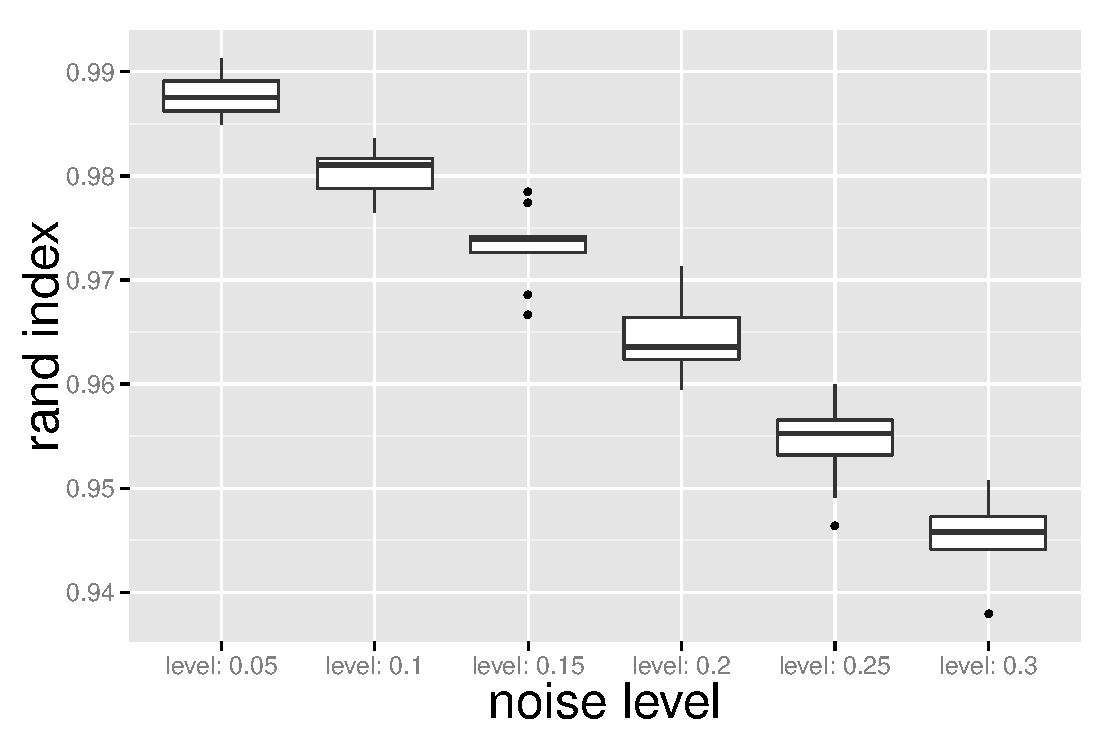
\includegraphics[width=\textwidth,height=0.8\textwidth]{fig/noise_boxplot_row.pdf}
    \subcaption{}
  \end{minipage}
  \begin{minipage}[t]{0.33\textwidth}
    \centering
    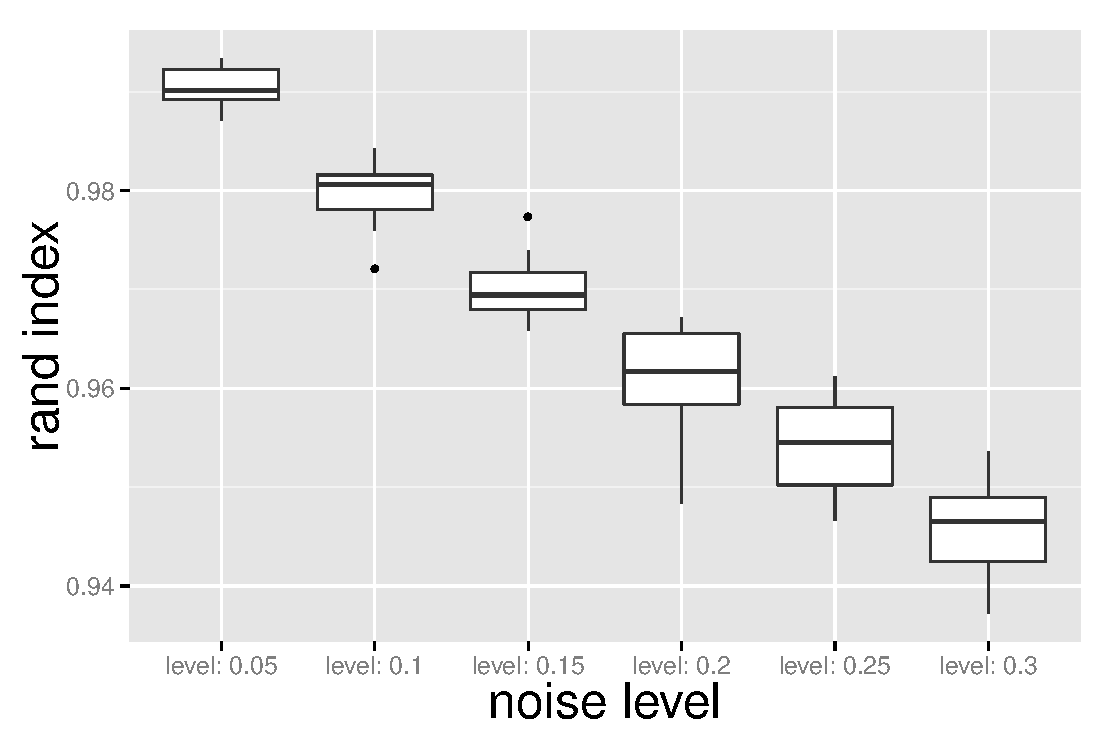
\includegraphics[width=\textwidth,height=0.8\textwidth]{fig/noise_boxplot_col.pdf}
    \subcaption{}
  \end{minipage}
  \begin{minipage}[t]{0.34\textwidth}
    \centering
    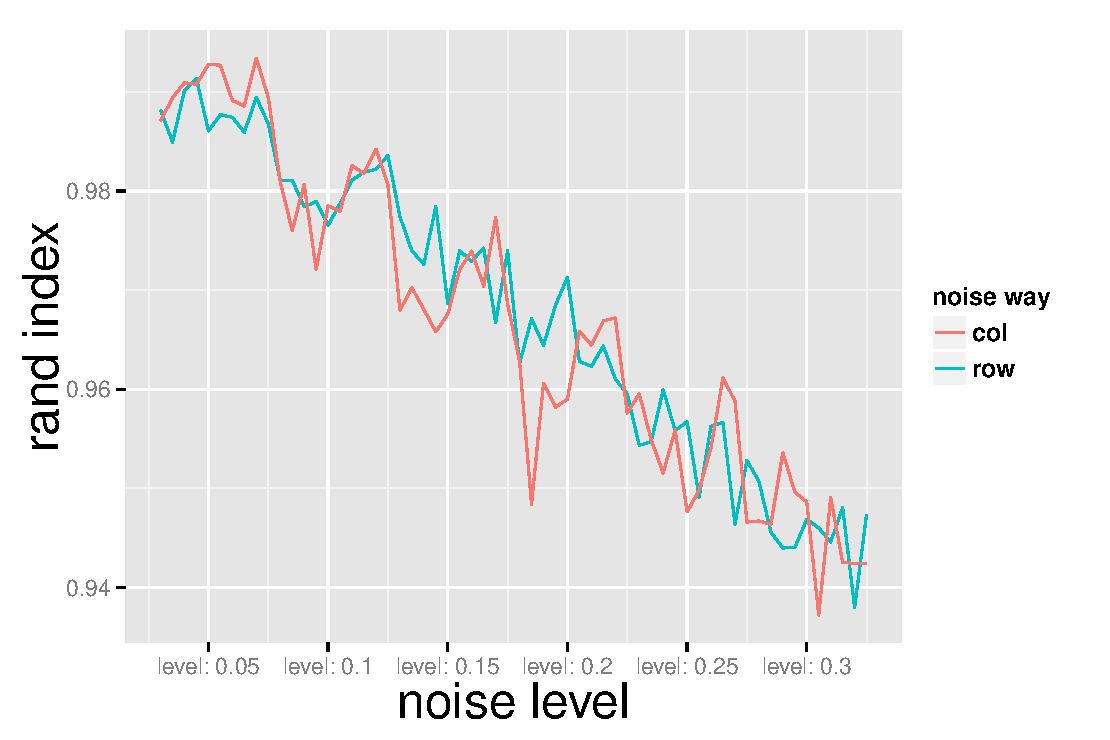
\includegraphics[width=\textwidth,height=0.8\textwidth]{fig/noise_line.pdf}
    \subcaption{}
  \end{minipage}
  \caption{\textbf{\textit{Rand Index} between the clustering of noised data and the raw data.} \textbf{(a)} Noises added on each row. \textbf{(b)}  Noises added on each column. \textbf{(c)}Average \textit{Rand Index} in terms of different levels of noises.}
  \label{fig:perturbation}
\end{figure*}

